\subsection{Ejercicio 2: Impacto de un Aumento en la Demanda Final}

En este ejercicio se evaluó cómo un aumento del 20\% en la demanda final del sector Agricultura afecta la producción total de todos los sectores de la economía de La Guajira.

\subsubsection{Demanda Final Original vs. Nueva}

\begin{table}[H]
\centering
\caption{Demanda Final Original vs. Nueva}
\begin{tabular}{lcc}
\toprule
Sector & Demanda Original & Demanda Nueva (+20\% Agricultura) \\
\midrule
Agricultura & 3.00 & 3.60 \\
Tecnología & 4.00 & 4.00 \\
Servicios & 8.00 & 8.00 \\
\bottomrule
\end{tabular}
\end{table}

\subsubsection{Producción Total Requerida: Original vs. Nueva}

\begin{table}[H]
\centering
\caption{Producción Total Requerida: Original vs. Nueva}
\begin{tabular}{lccc}
\toprule
Sector & Producción Original & Producción Nueva & Cambio (\%) \\
\midrule
Agricultura & 4.80 & 5.49 & +14.4\% \\
Tecnología & 7.88 & 8.04 & +2.0\% \\
Servicios & 11.70 & 11.83 & +1.1\% \\
\bottomrule
\end{tabular}
\end{table}

Los resultados muestran que el aumento del 20\% en la demanda de Agricultura genera un incremento del 14.4\% en su propia producción, del 2.0\% en el sector Tecnología y del 1.1\% en el sector Servicios. Esto demuestra el efecto multiplicador de la matriz de Leontief, donde un cambio en un sector se transmite a los demás a través de los encadenamientos productivos.

\begin{figure}[H]
\centering
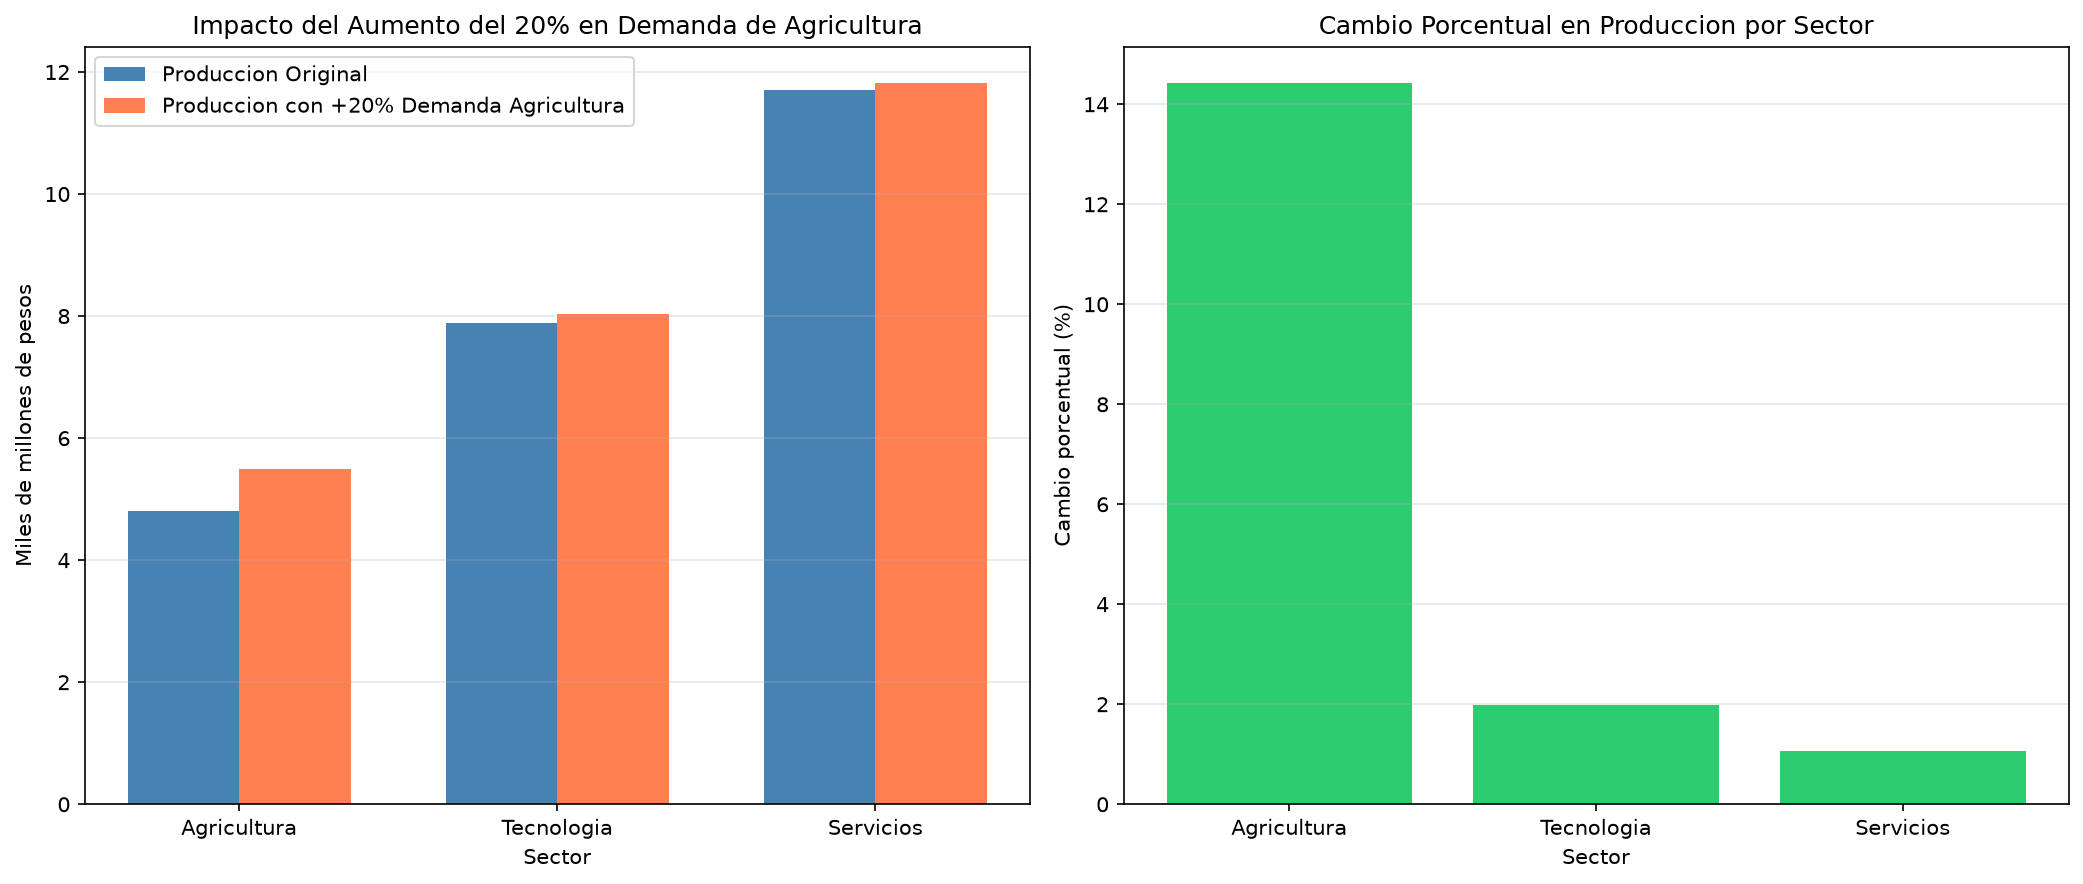
\includegraphics[width=0.9\textwidth]{ejercicio2_impacto_demanda/resultados_impacto.png}
\caption{Impacto del Aumento del 20\% en Demanda de Agricultura}
\end{figure}

\clearpage
